\documentclass{standalone}
\usepackage{tikz}
\usetikzlibrary{patterns, positioning}
\usepackage[sfdefault]{ClearSans} %% option 'sfdefault' activates Clear Sans as the default text font
\usepackage[T1]{fontenc}

\begin{document}
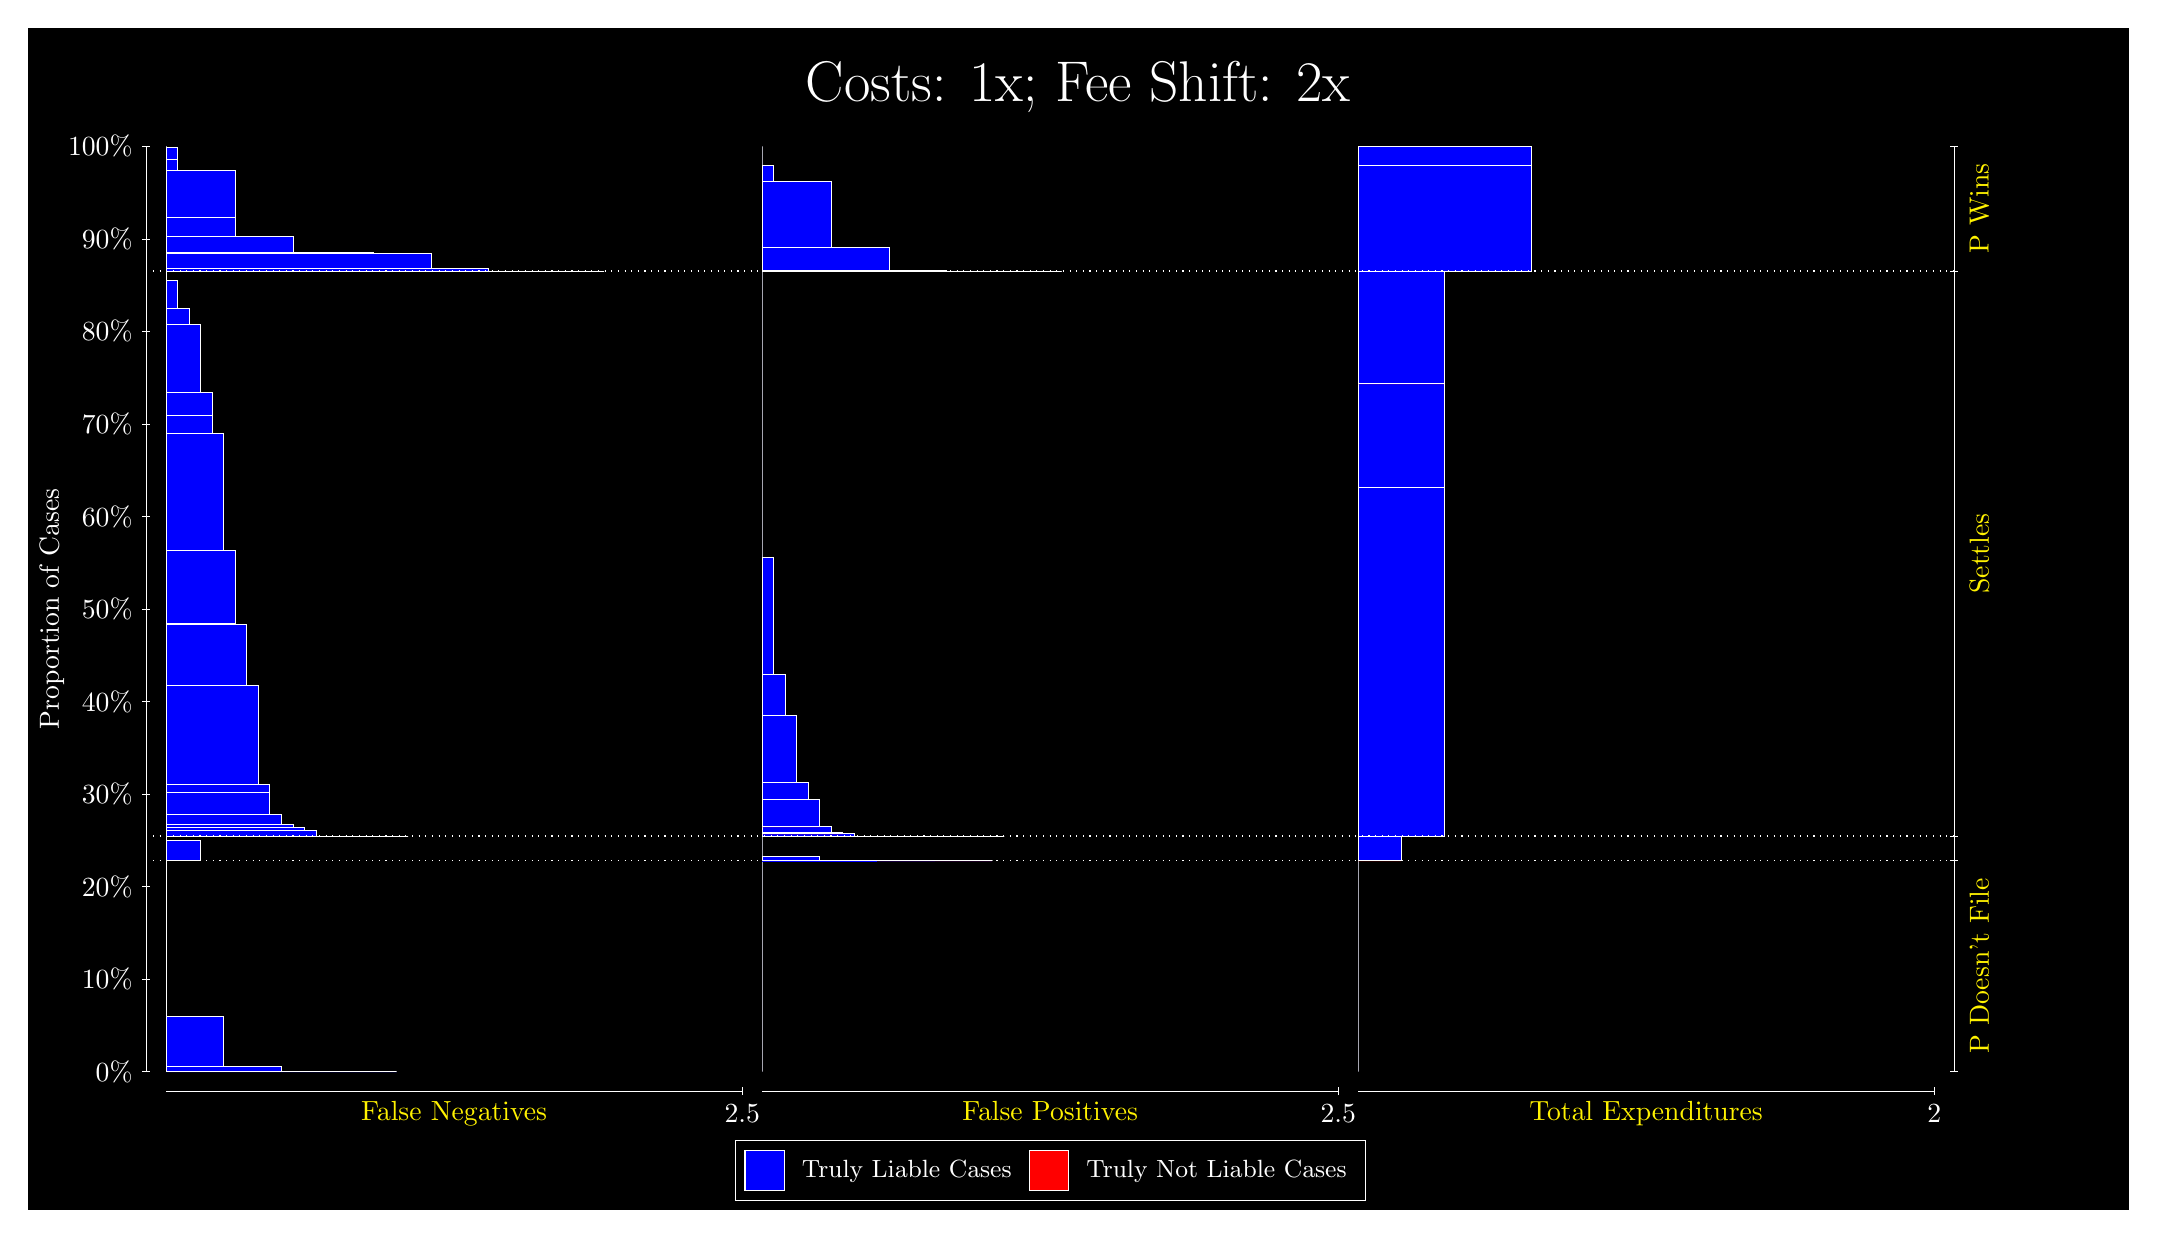
\begin{tikzpicture}
\draw[fill=black] (0,0) rectangle (26.667,15);
\draw[text=white] (0,13.5) rectangle (26.667,15) node[midway] {\huge Costs: 1x; Fee Shift: 2x};
\draw[white, very thin] (1.5,1.75) -- (1.5,13.5);
\node[rotate=90, text=white, anchor=center] at (0.3, 7.625) {Proportion of Cases};
\draw[white, very thin] (1.45,1.75) -- (1.55,1.75);
\node[text=white, anchor=east] at (1.45, 1.75) {0\%};
\draw[white, very thin] (1.45,2.925) -- (1.55,2.925);
\node[text=white, anchor=east] at (1.45, 2.925) {10\%};
\draw[white, very thin] (1.45,4.1) -- (1.55,4.1);
\node[text=white, anchor=east] at (1.45, 4.1) {20\%};
\draw[white, very thin] (1.45,5.275) -- (1.55,5.275);
\node[text=white, anchor=east] at (1.45, 5.275) {30\%};
\draw[white, very thin] (1.45,6.45) -- (1.55,6.45);
\node[text=white, anchor=east] at (1.45, 6.45) {40\%};
\draw[white, very thin] (1.45,7.625) -- (1.55,7.625);
\node[text=white, anchor=east] at (1.45, 7.625) {50\%};
\draw[white, very thin] (1.45,8.8) -- (1.55,8.8);
\node[text=white, anchor=east] at (1.45, 8.8) {60\%};
\draw[white, very thin] (1.45,9.975) -- (1.55,9.975);
\node[text=white, anchor=east] at (1.45, 9.975) {70\%};
\draw[white, very thin] (1.45,11.15) -- (1.55,11.15);
\node[text=white, anchor=east] at (1.45, 11.15) {80\%};
\draw[white, very thin] (1.45,12.325) -- (1.55,12.325);
\node[text=white, anchor=east] at (1.45, 12.325) {90\%};
\draw[white, very thin] (1.45,13.5) -- (1.55,13.5);
\node[text=white, anchor=east] at (1.45, 13.5) {100\%};

\draw[white, very thin] (24.457,1.75) -- (24.457,13.5);
\draw[white, very thin] (24.407,1.75) -- (24.507,1.75);
\node[anchor=west] at (24.407, 1.75) {};
\draw[white, very thin] (24.407,4.4284) -- (24.507,4.4284);
\node[anchor=west] at (24.407, 4.4284) {};
\draw[white, very thin] (24.407,4.7418) -- (24.507,4.7418);
\node[anchor=west] at (24.407, 4.7418) {};
\draw[white, very thin] (24.407,11.917) -- (24.507,11.917);
\node[anchor=west] at (24.407, 11.917) {};
\draw[white, very thin] (24.407,13.5) -- (24.507,13.5);
\node[anchor=west] at (24.407, 13.5) {};

\draw[white, very thin, fill=blue] (1.75,1.75) rectangle (4.6775,1.75);
\draw[white, very thin, fill=blue] (1.75,1.75) rectangle (3.9457,1.7505);
\draw[white, very thin, fill=blue] (1.75,1.7505) rectangle (3.2138,1.8146);
\draw[white, very thin, fill=blue] (1.75,1.8146) rectangle (2.4819,2.4492);
\draw[white, very thin, fill=red] (1.75,2.4492) rectangle (1.75,2.4492);
\draw[white, very thin, fill=blue] (1.75,2.4492) rectangle (1.75,4.4284);
\draw[white, very thin, fill=blue] (1.75,4.4284) rectangle (2.1891,4.6905);
\draw[white, very thin, fill=red] (1.75,4.6905) rectangle (1.75,4.6905);
\draw[white, very thin, fill=blue] (1.75,4.6905) rectangle (1.75,4.7418);
\draw[white, very thin, fill=blue] (1.75,4.7418) rectangle (4.8239,4.7418);
\draw[white, very thin, fill=blue] (1.75,4.7418) rectangle (4.5312,4.7418);
\draw[white, very thin, fill=blue] (1.75,4.7418) rectangle (4.2384,4.7418);
\draw[white, very thin, fill=blue] (1.75,4.7418) rectangle (4.092,4.7418);
\draw[white, very thin, fill=blue] (1.75,4.7418) rectangle (3.9457,4.7422);
\draw[white, very thin, fill=blue] (1.75,4.7422) rectangle (3.7993,4.7423);
\draw[white, very thin, fill=blue] (1.75,4.7423) rectangle (3.6529,4.816);
\draw[white, very thin, fill=blue] (1.75,4.816) rectangle (3.5065,4.8473);
\draw[white, very thin, fill=blue] (1.75,4.8473) rectangle (3.3602,4.8865);
\draw[white, very thin, fill=blue] (1.75,4.8865) rectangle (3.2138,5.013);
\draw[white, very thin, fill=blue] (1.75,5.013) rectangle (3.0674,5.2931);
\draw[white, very thin, fill=blue] (1.75,5.2931) rectangle (3.0674,5.3919);
\draw[white, very thin, fill=blue] (1.75,5.3919) rectangle (2.921,6.6495);
\draw[white, very thin, fill=blue] (1.75,6.6495) rectangle (2.7746,7.427);
\draw[white, very thin, fill=blue] (1.75,7.427) rectangle (2.6283,7.4481);
\draw[white, very thin, fill=blue] (1.75,7.4481) rectangle (2.6283,8.3711);
\draw[white, very thin, fill=blue] (1.75,8.3711) rectangle (2.4819,9.8608);
\draw[white, very thin, fill=blue] (1.75,9.8608) rectangle (2.3355,10.088);
\draw[white, very thin, fill=blue] (1.75,10.088) rectangle (2.3355,10.382);
\draw[white, very thin, fill=blue] (1.75,10.382) rectangle (2.1891,11.234);
\draw[white, very thin, fill=blue] (1.75,11.234) rectangle (2.0428,11.446);
\draw[white, very thin, fill=blue] (1.75,11.446) rectangle (1.8964,11.447);
\draw[white, very thin, fill=blue] (1.75,11.447) rectangle (1.8964,11.798);
\draw[white, very thin, fill=red] (1.75,11.798) rectangle (1.75,11.798);
\draw[white, very thin, fill=blue] (1.75,11.798) rectangle (1.75,11.917);
\draw[white, very thin, fill=blue] (1.75,11.917) rectangle (7.3123,11.917);
\draw[white, very thin, fill=blue] (1.75,11.917) rectangle (6.5805,11.917);
\draw[white, very thin, fill=blue] (1.75,11.917) rectangle (5.8486,11.95);
\draw[white, very thin, fill=blue] (1.75,11.95) rectangle (5.1167,12.141);
\draw[white, very thin, fill=blue] (1.75,12.141) rectangle (4.8239,12.141);
\draw[white, very thin, fill=blue] (1.75,12.141) rectangle (4.3848,12.152);
\draw[white, very thin, fill=blue] (1.75,12.152) rectangle (4.092,12.152);
\draw[white, very thin, fill=blue] (1.75,12.152) rectangle (3.6529,12.152);
\draw[white, very thin, fill=blue] (1.75,12.152) rectangle (3.3602,12.356);
\draw[white, very thin, fill=blue] (1.75,12.356) rectangle (2.921,12.356);
\draw[white, very thin, fill=blue] (1.75,12.356) rectangle (2.6283,12.601);
\draw[white, very thin, fill=blue] (1.75,12.601) rectangle (2.6283,13.202);
\draw[white, very thin, fill=blue] (1.75,13.202) rectangle (1.8964,13.334);
\draw[white, very thin, fill=blue] (1.75,13.334) rectangle (1.8964,13.485);
\draw[white, very thin, fill=red] (1.75,13.485) rectangle (1.75,13.485);
\draw[white, very thin, fill=blue] (1.75,13.485) rectangle (1.75,13.5);
\draw[white, very thin, fill=red] (9.3189,1.75) rectangle (9.3189,1.75);
\draw[white, very thin, fill=blue] (9.3189,1.75) rectangle (9.3189,4.4284);
\draw[white, very thin, fill=red] (9.3189,4.4284) rectangle (12.246,4.4284);
\draw[white, very thin, fill=blue] (9.3189,4.4284) rectangle (12.246,4.4284);
\draw[white, very thin, fill=blue] (9.3189,4.4284) rectangle (11.515,4.4284);
\draw[white, very thin, fill=blue] (9.3189,4.4284) rectangle (10.783,4.4288);
\draw[white, very thin, fill=blue] (9.3189,4.4288) rectangle (10.051,4.4797);
\draw[white, very thin, fill=blue] (9.3189,4.4797) rectangle (9.3189,4.7418);
\draw[white, very thin, fill=red] (9.3189,4.7418) rectangle (12.393,4.7418);
\draw[white, very thin, fill=blue] (9.3189,4.7418) rectangle (12.393,4.7418);
\draw[white, very thin, fill=red] (9.3189,4.7418) rectangle (11.807,4.7418);
\draw[white, very thin, fill=blue] (9.3189,4.7418) rectangle (11.807,4.7418);
\draw[white, very thin, fill=blue] (9.3189,4.7418) rectangle (11.661,4.7418);
\draw[white, very thin, fill=red] (9.3189,4.7418) rectangle (11.515,4.7418);
\draw[white, very thin, fill=blue] (9.3189,4.7418) rectangle (11.515,4.7418);
\draw[white, very thin, fill=red] (9.3189,4.7418) rectangle (11.222,4.7418);
\draw[white, very thin, fill=blue] (9.3189,4.7418) rectangle (11.222,4.7418);
\draw[white, very thin, fill=blue] (9.3189,4.7418) rectangle (11.075,4.7418);
\draw[white, very thin, fill=red] (9.3189,4.7418) rectangle (10.929,4.7418);
\draw[white, very thin, fill=blue] (9.3189,4.7418) rectangle (10.929,4.7419);
\draw[white, very thin, fill=blue] (9.3189,4.7419) rectangle (10.783,4.7419);
\draw[white, very thin, fill=red] (9.3189,4.7419) rectangle (10.636,4.7419);
\draw[white, very thin, fill=blue] (9.3189,4.7419) rectangle (10.636,4.7424);
\draw[white, very thin, fill=blue] (9.3189,4.7424) rectangle (10.49,4.772);
\draw[white, very thin, fill=red] (9.3189,4.772) rectangle (10.344,4.772);
\draw[white, very thin, fill=blue] (9.3189,4.772) rectangle (10.344,4.7891);
\draw[white, very thin, fill=blue] (9.3189,4.7891) rectangle (10.197,4.8603);
\draw[white, very thin, fill=red] (9.3189,4.8603) rectangle (10.051,4.8603);
\draw[white, very thin, fill=blue] (9.3189,4.8603) rectangle (10.051,5.2121);
\draw[white, very thin, fill=blue] (9.3189,5.2121) rectangle (9.9044,5.4248);
\draw[white, very thin, fill=blue] (9.3189,5.4248) rectangle (9.758,6.2768);
\draw[white, very thin, fill=blue] (9.3189,6.2768) rectangle (9.6116,6.7976);
\draw[white, very thin, fill=blue] (9.3189,6.7976) rectangle (9.4652,8.2873);
\draw[white, very thin, fill=blue] (9.3189,8.2873) rectangle (9.3189,11.917);
\draw[white, very thin, fill=red] (9.3189,11.917) rectangle (13.125,11.917);
\draw[white, very thin, fill=blue] (9.3189,11.917) rectangle (13.125,11.917);
\draw[white, very thin, fill=red] (9.3189,11.917) rectangle (12.393,11.917);
\draw[white, very thin, fill=blue] (9.3189,11.917) rectangle (12.393,11.917);
\draw[white, very thin, fill=red] (9.3189,11.917) rectangle (11.661,11.917);
\draw[white, very thin, fill=blue] (9.3189,11.917) rectangle (11.661,11.931);
\draw[white, very thin, fill=red] (9.3189,11.931) rectangle (10.929,11.931);
\draw[white, very thin, fill=blue] (9.3189,11.931) rectangle (10.929,12.215);
\draw[white, very thin, fill=blue] (9.3189,12.215) rectangle (10.197,13.061);
\draw[white, very thin, fill=red] (9.3189,13.061) rectangle (9.9044,13.061);
\draw[white, very thin, fill=blue] (9.3189,13.061) rectangle (9.9044,13.061);
\draw[white, very thin, fill=blue] (9.3189,13.061) rectangle (9.4652,13.265);
\draw[white, very thin, fill=red] (9.3189,13.265) rectangle (9.3189,13.265);
\draw[white, very thin, fill=blue] (9.3189,13.265) rectangle (9.3189,13.5);
\draw[white, very thin, fill=red] (16.888,1.75) rectangle (16.888,1.75);
\draw[white, very thin, fill=blue] (16.888,1.75) rectangle (16.888,4.4284);
\draw[white, very thin, fill=red] (16.888,4.4284) rectangle (17.437,4.4284);
\draw[white, very thin, fill=blue] (16.888,4.4284) rectangle (17.437,4.7418);
\draw[white, very thin, fill=red] (16.888,4.7418) rectangle (17.986,4.7418);
\draw[white, very thin, fill=blue] (16.888,4.7418) rectangle (17.986,9.1739);
\draw[white, very thin, fill=red] (16.888,9.1739) rectangle (17.986,9.1739);
\draw[white, very thin, fill=blue] (16.888,9.1739) rectangle (17.986,10.486);
\draw[white, very thin, fill=red] (16.888,10.486) rectangle (17.986,10.486);
\draw[white, very thin, fill=blue] (16.888,10.486) rectangle (17.986,11.917);
\draw[white, very thin, fill=red] (16.888,11.917) rectangle (19.083,11.917);
\draw[white, very thin, fill=blue] (16.888,11.917) rectangle (19.083,13.265);
\draw[white, very thin, fill=red] (16.888,13.265) rectangle (19.083,13.265);
\draw[white, very thin, fill=blue] (16.888,13.265) rectangle (19.083,13.5);
\draw[white, dotted] (1.5,4.4284) -- (24.457,4.4284);
\draw[white, dotted] (1.5,4.7418) -- (24.457,4.7418);
\draw[white, dotted] (1.5,11.917) -- (24.457,11.917);
\draw[white, very thin] (1.75,1.5) -- (9.0689,1.5);
\node[text=yellow, anchor=north] at (5.4094, 1.5) {False Negatives};
\draw[white, very thin] (9.0689,1.45) -- (9.0689,1.55);
\node[text=white, anchor=north] at (9.0689, 1.45) {2.5};

\draw[white, very thin] (9.3189,1.5) -- (16.638,1.5);
\node[text=yellow, anchor=north] at (12.978, 1.5) {False Positives};
\draw[white, very thin] (16.638,1.45) -- (16.638,1.55);
\node[text=white, anchor=north] at (16.638, 1.45) {2.5};

\draw[white, very thin] (16.888,1.5) -- (24.207,1.5);
\node[text=yellow, anchor=north] at (20.547, 1.5) {Total Expenditures};
\draw[white, very thin] (24.207,1.45) -- (24.207,1.55);
\node[text=white, anchor=north] at (24.207, 1.45) {2};

\node[text=yellow, centered, rotate=90] at (24.777, 3.0892) {P Doesn't File};

\node[text=yellow, centered, rotate=90] at (24.777, 8.3292) {Settles};
\node[text=yellow, centered, rotate=90] at (24.777, 12.708) {P Wins};

\draw (12.978300999999998,1.5) node[draw=none] (baseCoordinate) {};
\begin{scope}[align=center]
        \matrix[scale=0.5, draw=white, below=0.5cm of baseCoordinate, nodes={draw}, column sep=0.1cm]{
            \node[rectangle, draw, minimum width=0.5cm, minimum height=0.5cm, fill=blue] {}; &
            \node[draw=none, font=\small, text=white] (B) {Truly Liable Cases}; &
            \node[rectangle, draw, minimum width=0.5cm, minimum height=0.5cm, fill=red] {}; &
            \node[draw=none, font=\small, text=white] (B) {Truly Not Liable Cases}; \\
            };
\end{scope}

\end{tikzpicture}
\end{document}